\begin{minipage}{75mm}
Returns a vector with the vertices of a polygon with everything to the left of the line going from s to e cut away.
\end{minipage}
\begin{minipage}{15mm}
\vspace{-6mm}
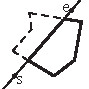
\includegraphics[width=\textwidth]{../code/Geometry/Polygon/PolygonCut}
\vspace{-6mm}
\end{minipage}
\begin{minted}[breaklines = true,
    breakanywhere = true,
    frame=lines,    
    fontfamily=tt,
    linenos=false,
    numberblanklines=true,
    numbersep=2pt,
    gobble=0,
    framerule=1pt,
    framesep=1mm,
    funcnamehighlighting=true,
    tabsize=1,
    obeytabs=false,
    mathescape=false
    samepage=false, %with this setting you can force the list to appear on the same page
    showspaces=false,
    showtabs =false,
    texcl=false]{C++}
/* Usage:
 *  vector<P> p = ...;
 *  p = polygonCut(p, P(0,0), P(1,0));
 * Status: tested but not extensively
 */
#include "Point.h"
#include "lineIntersection.h"

typedef Point<double> P;
vector<P> polygonCut(const vector<P>& poly, P s, P e) {
  vector<P> res;
  rep(i,0,sz(poly)) {
    P cur = poly[i], prev = i ? poly[i-1] : poly.back();
    bool side = s.cross(e, cur) < 0;
    if (side != (s.cross(e, prev) < 0))
      res.push_back(lineInter(s, e, cur, prev).second);
    if (side)
      res.push_back(cur);
  }
  return res;
}
\end{minted}
